
\section{Results}

Figure~\ref{fig:results} shows the best, average, and worst genome fitness in the population over 2000 generations. Since the optimal fitness value is zero, and larger fitness values mean a ``worse'' genome, we negate every fitness value to obtain a more intuitive graph with zero at the top. Results seem fairly typical for a genetic algorithm. Average and worst fitness values are messy and have a high variance across generations. The best fitness values converge fairly quickly. After around 1000 generations, the best fitness is around -300. Improvements slow down after the first 1000 generations, but usually end up between 0 and -100 after the full 2000 generations. For a $100 \times 100$ grid, any fitness value under 100 is very good considering the worst fitness values may reach -10,000. This behaviour is fairly consisten over multiple executions of the evolutionary algorithm.

% \begin{figure}[h]
%     \centering
%     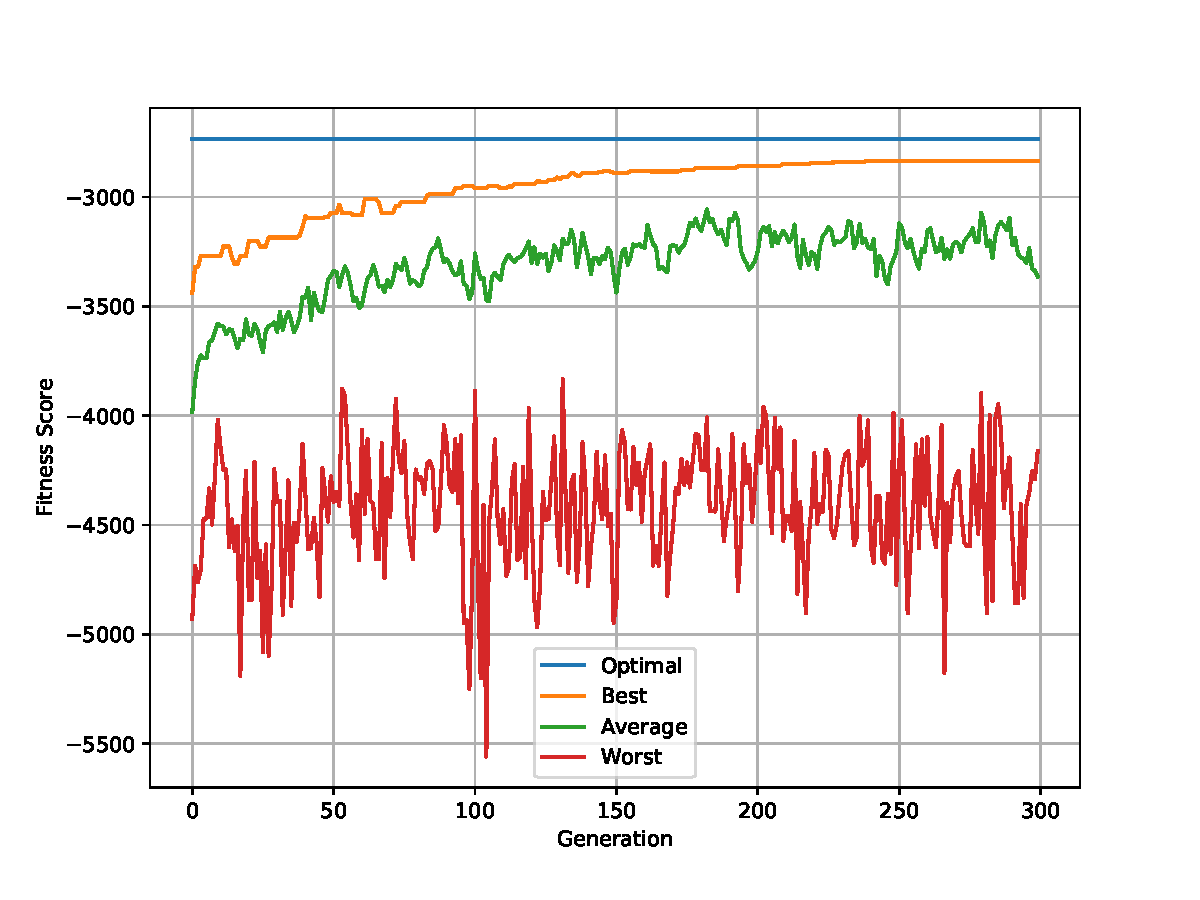
\includegraphics[scale=0.75]{figures/results.pdf}
%     \caption{ \small Fitness results over 2000 generations.}
%     \label{fig:results}
% \end{figure}
